\documentclass[11pt,a4paper]{article}
\usepackage[utf8]{inputenc}
\usepackage[T1]{fontenc}
\usepackage[english]{babel}
\usepackage{lmodern,microtype,amsmath,amssymb,booktabs,array,graphicx,xcolor,geometry,setspace,float,longtable}
\usepackage{tikz}
\usetikzlibrary{arrows.meta,positioning}
\usepackage[font=small,labelfont=bf]{caption}
\usepackage[hidelinks]{hyperref}
\geometry{margin=25mm}
\setstretch{1.16}
\setlength{\parskip}{0.35em}
\setlength{\parindent}{1.2em}
\setlength{\emergencystretch}{2em}
\makeatletter
\setlength{\@fptop}{0pt}
\setlength{\@fpsep}{18pt}
\setlength{\@fpbot}{0pt plus 1fil}
\makeatother
\definecolor{reused}{HTML}{1755A0}
\definecolor{revised}{HTML}{B85A00}
\definecolor{added}{HTML}{B02228}
\newcommand{\old}[1]{{\color{reused}#1}}
\newcommand{\rev}[1]{{\color{revised}#1}}
\newcommand{\new}[1]{{\color{added}#1}}
\newenvironment{addition}{\begingroup\color{added}}{\endgroup}
\newcommand{\pp}{percentage points}
\newcommand{\figroot}{../../3. Output/two_papers_2026-09-22/figures/}
\newcommand{\draftlegend}{\begin{center}\small\color{black}Coauthor working draft --- 22 September 2026\\\old{Blue: wording retained verbatim.}\quad\rev{Orange: revised existing material.}\\\new{Red: new text or analysis.} Figure frames and captions indicate provenance; plotted colors do not.\end{center}}
\newcommand{\authors}{\old{Ignacio Garijo-Campos} \and \old{Antonio Alfonso} \and \old{Pablo Bra\~nas-Garza} \and \old{Diego Jorrat} \and \old{Angel Sanchez}}
\newcommand{\plot}[4]{\begin{figure}[!htbp]\centering\begingroup\color{#1}\setlength{\fboxsep}{2pt}\fbox{\includegraphics[width=.94\linewidth]{\figroot#2.png}}\caption{\textcolor{#1}{#3}}\label{#4}\endgroup\end{figure}}
\newcommand{\tabnote}[1]{\par\smallskip{\footnotesize\noindent\textit{Notes:} #1\par}}
\newcommand{\inputtab}[4]{\begin{table}[!htbp]\centering\begingroup\color{#1}\caption{\textcolor{#1}{#3}}\label{#4}\small\input{tables/#2.tex}\endgroup\end{table}}
\date{}
\renewcommand{\floatpagefraction}{0.8}
\renewcommand{\topfraction}{0.9}
\renewcommand{\textfraction}{0.07}
\makeatletter\newcommand{\sectionfloatbarrier}{\ifx\@deferlist\@empty\else\clearpage\fi}\makeatother

\title{\rev{Shared Academic Criteria and Systematic Disagreement in Teachers' Grade-Repetition Recommendations}}
\author{\authors}
\begin{document}
\maketitle\draftlegend
\color{revised}
\begin{abstract}\color{added}
Teachers can agree about the importance of academic difficulties while disagreeing about whether a particular student should repeat a grade. We study that distinction using 22,124 recorded recommendations from 2,705 teachers in a regional survey experiment in Spain. Within-teacher differences are dominated by failed subjects and low basic competences, with evidence that the two signals reinforce each other. Disagreement is concentrated where they conflict: for profiles with many failed subjects but adequate competences, two respondents disagree in 49.1 percent of same-profile pairs. Between-teacher dispersion is also systematic within the task. Its variance is 2.11 times a benchmark that redistributes responses within identical cards and assignment contexts while preserving teachers' exposures. Yet professional characteristics and reported beliefs explain little of this variation. Nested validation on 2,156 complete cases yields out-of-fold $R^2$ values of 3.06 percent for a linear model, 3.01 percent for ridge regression, and 1.48 percent for a tuned random forest. The results locate a consequential boundary in teachers' application of shared academic criteria, while showing why detectable group associations provide a weak basis for predicting an individual teacher's relative recommendation propensity.

\end{abstract}
\noindent\textbf{Keywords:} grade repetition; teacher judgment; standardized vignettes; disagreement; prediction; educational inequality.

\section{Introduction}
Grade-repetition recommendations translate several kinds of evidence into a binary educational judgment. Failed subjects may indicate that a student has not met the requirements for progression. Basic competences provide a partly different signal of what the student can do. Attendance, classroom behavior, and background can further shape how a teacher interprets the difficulty. Even when teachers broadly agree that academic performance should matter, they may disagree about how much evidence is enough, which evidence should take precedence, and whether repetition is an appropriate response.

Understanding this disagreement requires more than comparing raw repetition rates across classrooms. A teacher who recommends repetition frequently may teach students with greater difficulties. Conversely, teachers facing similar cases may apply different decision thresholds or interpret the same signals differently. Standardized student profiles make the information under evaluation comparable. They allow us to ask both which attributes organize recommendations and where comparable information leaves room for divergent judgments.

Research on the consequences of retention offers no universal decision rule that resolves these cases. Estimated effects vary with research design, institutional setting and the students compared \cite{allen,goos}. Research on teachers' beliefs and judgments establishes that their interpretations also matter \cite{tomchin,bonvin,klapproth}. The remaining empirical challenge is to connect the common structure of recommendations to the distribution of disagreement across cases and across teachers. A large average response to failed subjects does not tell us whether teachers agree when grades and competences point in different directions.

We use a survey experiment with primary and secondary teachers in Castilla-La Mancha, Spain. The retained data contain 22,124 recommendations from 2,705 teachers evaluating recorded profiles with six coded attributes. Our analysis proceeds from the decision to the decision-maker. First, we estimate within-teacher attribute contrasts and examine conflicting academic signals. Second, we measure disagreement about identical cards and compare the dispersion of teachers' relative recommendation propensity with an exchangeability benchmark. Third, we ask how well professional characteristics and reported beliefs predict that propensity for held-out teachers.

\new{This sequence distinguishes three empirical possibilities. Shared attribute responses can coexist with case-specific disagreement. That disagreement can cluster within teachers rather than being distributed as independent responses across otherwise comparable cases. Finally, systematic within-task differences can still be difficult to predict from the available covariates. The second proposition is especially important: a low predictive $R^2$ should not be used as evidence that there is no respondent-level structure to explain.}

The results support all three distinctions. Failed subjects and low competences have the largest additive within-teacher coefficients, 54.6 and 27.1 percentage points. An interaction model indicates that low competences add more to repetition recommendations when several subjects are failed. Nevertheless, the profile category combining many failed subjects with adequate competences divides respondents almost evenly. Its same-profile disagreement rate is 49.1 percent, compared with 5.8 percent where neither academic difficulty is present.

\new{The dispersion of teachers' relative propensity is not reproduced by shuffling answers among respondents who received the same recorded card in the same assignment context. Observed variance is 2.11 times the average permuted variance; the finding remains among teachers with at least eight responses and within the control context. This is evidence of concentration within the survey encounter, without establishing a persistent trait across time. Observable teacher information nonetheless has limited predictive value. Nested validation gives a mean $R^2$ of 3.06 percent for the full linear model; neither regularization nor a tuned forest uncovers a large predictive gain.}

Our contribution is therefore not simply that academic performance matters or that teachers differ. It is to locate the academic cases that divide judgment, demonstrate an internal respondent-level structure to the disagreement, and assess how far common teacher descriptors can anticipate it. These results identify a substantive boundary of shared decision criteria while avoiding a typology inferred solely from significant regression coefficients. The recommendations concern hypothetical cases; their appropriateness and their consequences for students are separate questions.

\section{Related literature}
The first relevant literature concerns the consequences of retaining a student. Allen et al.\ \cite{allen} find that stronger research designs yield less negative retention effects than weaker designs. Goos et al.\ \cite{goos} document substantial heterogeneity across settings and methods in a broad review. These findings motivate studying how teachers evaluate repetition, but they do not supply a single correct answer to every vignette. The present outcome is a recommendation, not the causal effect of retention on later achievement.

A second literature investigates teachers' beliefs and judgments. Tomchin and Impara \cite{tomchin} examine the reasoning teachers use to justify retention. Bonvin \cite{bonvin} relates teacher attitudes and judgments to actual retention decisions. These studies establish that teachers' interpretations deserve attention alongside student performance. More recently, Klapproth and Beyte \cite{klapproth} use experimental vignettes to study grade-point averages, gender, failed subjects, and teacher attitudes. Their work is a close antecedent: experimental analysis of retention recommendations is not itself new. Our extension connects conflicting academic signals, respondent-level concentration of disagreement, and a separate test of out-of-sample predictability in a larger teacher sample. The same evidence can therefore distinguish a common decision pattern from the ability to anticipate individual departures from it.

The distinction between beliefs, knowledge, and reported attitudes also matters \cite{pajares}. An association between a belief item and a recommendation does not show that changing the belief would change the decision. Here, several belief measures follow the decision task. We therefore use them to characterize and predict responses rather than as randomized explanations of behavior.

\new{Methodologically, the study draws on the logic of multidimensional vignette experiments \cite{conjoint}. Interpretation depends on the profiles actually represented and the distribution over which a comparison is averaged. Standardizing information strengthens internal comparisons, but external validity requires separate evidence. Validation of vignette choices against real behavior in other domains \cite{validation} does not validate retention recommendations automatically. Finally, the distinction between fitting associations and predicting new observations motivates our validation procedure \cite{prediction}. Random forests \cite{rf} provide a flexible comparison, and SHAP summaries \cite{shap} describe the fitted prediction function rather than the causal importance of teacher characteristics.}

\section{Study design and measurement}
\subsection{Participants and recommendation task}
The study concerns primary and secondary teachers in Castilla-La Mancha, Spain. The initial study plan specifies recruitment through the regional education authority and schools forwarding an online survey to teachers. Participation is voluntary, so a broad invitation frame does not imply a probability sample of responding teachers. The raw export contains 4,942 records; the retained cleaned file contains 4,553, and 2,705 contribute at least one usable recommendation. Records without an outcome cannot characterize recommendation propensity.

The survey combines an initial questionnaire on professional and demographic characteristics, examples explaining the task, eight intended experimental cards, and a final questionnaire on beliefs and perceived educational resources. Figure~\ref{fig:timelineA} distinguishes the timing of baseline characteristics and later belief reports. The response on each card is a binary choice between promotion and repetition. Complex background is the construct used in the present analysis; it is not interpreted as migrant status.

\old{Before the task, teachers are shown two examples. One is an ideal student with no negative characteristics. The other is a student with all characteristics associated with grade repetition. These examples were included to make the task clear and to work as an attention check. We removed teachers that failed the student with none of the characteristics associated with grade repetition. We decided not to remove teachers that did not fail the student with all before-mentioned characteristics, since there are teachers that do not believe in grade repetition at all.}

The analysis preserves the original retained-response definition. The two favorable-example fields are excluded, while the other recorded card responses remain informative observations. The number of retained responses therefore need not equal eight: 1,736 teachers contribute nine, 633 contribute eight, and 336 contribute between one and seven. These are recorded recommendations, including retained example information; they are not relabeled as nine experimental tasks. When a question identifier is reused, the export does not provide two separate answers that can be reliably recovered by relabeling the column.

\begin{figure}[!htbp]\centering\color{added}
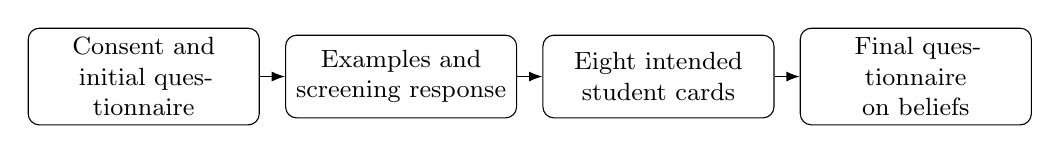
\begin{tikzpicture}[n/.style={draw,rounded corners,align=center,text width=2.7cm,minimum height=1.05cm,font=\small},>=Latex]
\node[n] (a) {Consent and\\initial questionnaire};
\node[n,right=0.32cm of a] (b) {Examples and\\screening response};
\node[n,right=0.32cm of b] (c) {Eight intended\\student cards};
\node[n,right=0.32cm of c] (d) {Final questionnaire\\on beliefs};
\draw[->] (a)--(b);\draw[->] (b)--(c);\draw[->] (c)--(d);
\end{tikzpicture}
\caption{\new{Timing of the measurements used in this paper. One survey encounter contains several modules; the diagram does not represent longitudinal waves. The shared study context is disclosed in Appendix~\ref{app:scope}.}}\label{fig:timelineA}
\end{figure}

\subsection{Recorded profile support and covariates}
The six binary characteristics are coded using the existing study vectors. The 64 possible identifiers represent 56 distinct attribute combinations under that coding. We retain this support rather than reconstruct unobserved profiles or treat every identifier as an independently randomized combination. Appendix~\ref{app:support} documents the implications. The within-teacher regression is consequently reported as an additive summary over the observed support. Its interpretation as a marginal causal attribute effect requires the relevant assignment and support assumptions; the existence of six binary variables alone does not establish those assumptions.

The baseline predictor set, $X_1$, contains educational stage, experience, tenure at the current school, gender, age, school ownership, a reported permanent public appointment indicator, and number of teaching groups. $X_2$ adds perceived teacher impact, self-reported empathy, and the effort-versus-luck item. The final specification adds the resource-skepticism composite. Larger values on the effort item indicate a stronger role attributed to effort. The resource composite averages standardized responses about excessive resources allocated to repeaters and ineffective additional resources, and is standardized again. Its two items correlate at 0.483 in the available observations; the composite summarizes related judgments rather than establishing a single validated latent construct.

We retain the existing harmonization of instrument versions: alternative impact items are combined, and empathy responses on the longer scale are mapped to the five-category scale. Age and experience enter jointly because the target is their conditional association. The public-employment item is described according to what was actually recorded; absence of a public appointment report is not evidence of a temporary private-sector contract.

\section{Decision framework and empirical strategy}
\begin{addition}
\subsection{Common information, differing judgments}
Let $x$ denote the information on a student profile and let $V_j(x)$ be teacher $j$'s perceived net educational value of recommending repetition rather than promotion. A simple representation is
\[
 Y_j(x)=\mathbf{1}\{V_j(x)+u_j(x)>0\}.
\]
Differences in $V_j(x)$ may arise from expected learning gains, perceived costs, beliefs about alternatives, or different interpretations of the same information. The term $u_j(x)$ accommodates response noise and omitted considerations. The framework is deliberately agnostic about whether disagreements are justified. It motivates three separate empirical objects: changes across presented attributes, disagreement at a given profile, and the predictability of a teacher's average response relative to comparable cases.

For a specified profile distribution $Q$, a population target could be written as
\[
 \theta_j(Q)=E_{x\sim Q}\{p_j(x)-\bar p(x)\},
\]
where $p_j(x)$ is a recommendation probability and $\bar p(x)$ is the comparison-population average. This target depends on both the reference population and $Q$. The available task estimates a finite-response analogue over each teacher's recorded cases. It does not identify $p_j(x)$ for all profiles or a context-free personal trait.
\end{addition}

\subsection{Attribute coefficients and same-profile disagreement}
At the card level, we estimate
\[
 Y_{ij}=\alpha_j+X_{ij}'\beta+\varepsilon_{ij},
\]
where $\alpha_j$ is a teacher fixed effect and $X_{ij}$ contains the six attributes. Each coefficient compares responses within teachers while adjusting for the other recorded attributes. Standard errors are clustered by teacher. The model uses 22,006 observations from 2,587 teachers; the 118 single-response teachers contribute no within-teacher variation. We retain the linear probability specification to report all coefficients in percentage points.

\new{Disagreement is measured separately from this regression. For a card with $n_i$ responses and $s_i$ recommendations to repeat, the probability that two distinct observed respondents disagree is $D_i=2s_i(n_i-s_i)/[n_i(n_i-1)]$. We average $D_i$ using observed card frequencies, and also report equal-identifier weighting. This is disagreement about an identical recorded card, not unexplained variance from a linear model. It is descriptive of the respondents and survey context.}

\subsection{Relative recommendation propensity}
\old{The preferred measure defines harshness as the average deviation from other teachers who evaluated the same card. We define it in two steps. First, for each teacher-card decision, we compute the distance between teacher \(j\)'s decision for card \(i\) and the leave-one-out repetition rate for that same card:}
\old{\[
d_{ij}=R_{ij}-\bar{R}_{i,-j}.
\]}
\old{Here, \(R_{ij}\) equals one if teacher \(j\) recommends repetition for card \(i\), and zero otherwise. The term \(\bar{R}_{i,-j}\) is the average repetition rate for card \(i\) among all other teachers who evaluated that same card, excluding teacher \(j\). Second, we average those distances across the cards evaluated by teacher \(j\):}
\old{\[
H^b_j=\frac{1}{n_j}\sum_{i\in I_j} d_{ij}.
\]}
We refer to $H^b_j$ as relative recommendation propensity. A value of 0.10 indicates an average recommendation ten percentage points above the leave-one-out rate for the recorded cards. The historical label ``harshness'' does not imply a normative judgment about whether repetition was appropriate.

\new{The index has useful limits and properties. It lies in $[-1,1]$; excludes the focal response from its comparison rate; and satisfies $\sum_j n_j H^b_j=0$ exactly when each recorded teacher-card response appears once. Its unweighted teacher mean need not be zero when response counts differ. Adjusting for card averages improves comparability but does not equalize measurement precision or remove sampling noise. We report teacher-level regressions with HC3 covariance and supplement their uncertainty with 399 teacher bootstrap draws that reconstruct the reference rates.}

We retain terciles of the observed index as a descriptive display. Ties produce groups of 908, 864, and 933 teachers. Because these groups are defined using the same decisions subsequently described, the resulting slopes do not independently validate latent types or estimate the effect of becoming more repetition-prone.

\begin{addition}
\subsection{Is disagreement concentrated within teachers?}
The dispersion of $H^b_j$ contains both respondent-level structure and variation due to observing a limited set of binary decisions. To distinguish these, we redistribute answers among teachers within the same recorded card and assignment cell. Every teacher retains the same cards and number of observations; each card--context stratum retains its number of repetition recommendations. What is broken is the association between a particular teacher and that teacher's answers across cards.

For each of 1,999 permutations, we reconstruct the score and calculate its variance across teachers. We compare the observed variance with this conditional reference, reporting the ratio and the proportion of permutations with at least as much dispersion. We repeat the entire exercise among teachers with at least eight recorded responses and in the no-policy-assignment control. Each restricted sample uses its own card reference population. The exercise asks whether responses are exchangeable across teachers under these conditioning variables. It does not estimate temporal reliability or distinguish every possible source of within-teacher dependence.

\subsection{Conflicting signals and prediction}
We cross failed subjects with basic competences to form four observed academic categories. Their recommendation rates use teacher-clustered intervals. Same-profile disagreement is first calculated within exact identifiers and then averaged within the category. Because other attributes have different distributions across categories, these rates are descriptions of observed cases. A separate teacher fixed-effect model adds three interactions of failed subjects with competences, absence and discipline to the six main attributes. Holm adjustment covers these three interaction tests. The model tests departures from the additive summary over the retained support.

Prediction uses five repetitions of five outer teacher folds. On the common sample of 2,156 complete cases, we compare a training-mean baseline, OLS with $X_1$, $X_2$ and $X_3$, and ridge and forest models using $X_3$. We separately evaluate baseline-only models on their available sample of 2,641 teachers. In every split, the training target uses training-only leave-one-out card rates; test targets subtract the training card means. A test teacher never contributes to its reference population or the fitting of its predictor.

The ridge penalty and forest settings are selected by three inner teacher folds, wholly within each outer training set. Card references and resource standardization are rebuilt at the inner level as well. Forest tuning considers two candidate-variable counts and three minimum node sizes; final fits use 500 trees. Ridge considers ten penalties after training-based predictor scaling. Appendix~\ref{app:prediction} gives the complete specification. Performance is
\[
R^2_{\mathrm{test}}=1-\frac{\sum_j(H_j^{\mathrm{test}}-\widehat H_j)^2}{\sum_j(H_j^{\mathrm{test}}-\overline H_{\mathrm{train}(j)})^2}.
\]
We report partition-averaged RMSE, $R^2$, and paired loss differences. An overlap-corrected approximation assesses the uncertainty of comparisons across the 25 outer test folds \cite{nadeau}; partition ranges alone are not confidence intervals. Held-out SHAP and permutation loss describe the tuned forest's use of the covariates rather than their causal effects.
\end{addition}

\section{Results}
\subsection{Academic information dominates the average recommendation}
Table~\ref{tab:attrA} reports the within-teacher coefficients. Three or more failed subjects have a coefficient of 54.62 points (95 percent interval 53.23 to 56.01); low basic competences have a coefficient of 27.07 (25.83 to 28.31). Frequent unjustified absence and serious disciplinary problems have smaller positive coefficients, 6.37 and 4.56 points respectively. A complex background is associated with a 1.88-point reduction conditional on the other attributes. The male-student coefficient is 0.26 points, with an interval from $-0.62$ to 1.15. This supports a small average gender contrast in the coded task, rather than the absence of every possible gender interaction.
\inputtab{revised}{A_attributes}{Within-teacher student-attribute coefficients}{tab:attrA}
The sizes distinguish the role of academic signals from behavioral and background information. They do not establish the optimal weights for actual educational decisions. Nor does the negative background coefficient identify empathy as a mechanism: different beliefs about causes, alternatives, or the costs of repetition can generate the same sign. The restricted no-scenario comparison in Appendix~\ref{app:scope} yields similar dominant academic coefficients.

\subsection{The disagreement boundary lies between grades and competences}
\begin{addition}
Table~\ref{tab:academicA} locates the aggregate disagreement. Only 3.0 percent of recommendations favor repetition when the profile has few failed subjects and adequate competences. With low competences but few failures, the share rises to 23.8 percent. With many failures but adequate competences, it is 51.5 percent. When both difficulties occur, it reaches 85.5 percent. The asymmetry shows that low competences and failed subjects are not interchangeable signals in the recorded judgments.
\end{addition}
\inputtab{added}{A_academic}{Conflicting academic signals and same-profile disagreement}{tab:academicA}
\begin{addition}
The disagreement figures sharpen this comparison. Where many failures coexist with adequate competences, the probability that two distinct teachers evaluating the same identifier disagree is 49.1 percent. This is close to the maximum of a balanced binary choice, and much larger than the 5.8 percent for profiles with neither academic difficulty. The other two categories yield 35.6 and 24.7 percent disagreement. These are averages of within-identifier disagreement, so they do not merely compare different profiles grouped under the same academic label.

In the interaction specification, failed subjects and low competences reinforce one another: the interaction is 10.56 points (95 percent interval 8.17 to 12.95), remaining clear after the three-test Holm adjustment. The low-competence coefficient is 21.66 points when the failed-subject indicator is zero and 32.22 points when it is one. Interactions with absence and discipline are much smaller and uncertain. Table~\ref{tab:interactionsA} reports the full specification.

This pattern is consistent with a cumulative use of academic evidence on the probability scale: the marginal association of one academic difficulty is larger in the presence of the other. It does not uniquely establish a psychological decision rule; a nonlinear response to an underlying threshold can produce a similar interaction. The substantive point is that agreement is greatest when the academic signals align, while failed subjects with adequate competences mark a contested decision boundary. The experiment has no measure establishing which recommendation at that boundary is educationally correct.
\end{addition}
\inputtab{added}{A_interactions}{Academic complementarities in within-teacher recommendations}{tab:interactionsA}

\subsection{Comparable cases still generate disagreement}
The overall recorded repetition rate is 47.62 percent when decisions receive equal weight; the teacher-weighted average is 48.39 percent. The frequency-weighted probability of a disagreement between distinct teachers evaluating the same identifier is 25.89 percent, compared with 26.01 percent under equal-identifier weighting. Consequently, a clear aggregate hierarchy does not mean that individual recommendations coincide.

The relative-propensity distribution has a standard deviation of 20.97 points and an unweighted mean of $-0.61$ points. Figure~\ref{fig:distributionA} shows the distribution without imposing normality. There are 169 teachers whose retained responses never recommend repetition. That observed pattern is compatible with several explanations, including opposition to repetition, the cases observed, or limited response counts; it is not itself a measurement of a general belief.
\plot{revised}{propensity_distribution}{Distribution of relative recommendation propensity among 2,705 teachers. The distribution combines differing numbers of recorded responses.}{fig:distributionA}
Tercile summaries preserve an intuitive description of the sample (Appendix~\ref{app:terciles}). Teachers in the lower and upper groups recommend repetition on 25.87 and 70.13 percent of their recorded cases, respectively. Their average ages are 46.27 and 44.22 years. These summaries show differences in the realized responses and modest shifts in some characteristics; the large response contrast is partly built into how the groups are formed.

\subsection{Disagreement has a respondent-level structure within the task}
\begin{addition}
The observed score SD is 20.97 points. Under the response-redistribution benchmark, the square root of average variance is 14.45 points; the central 95 percent range of permuted SDs is 13.76--15.18 points. Observed variance is 2.11 times the reference variance, and none of the 1,999 permutations reaches it ($p=0.0005$ using the plus-one correction). Thus finite binary responses and the observed exposures do not reproduce the dispersion under this conditional exchangeability benchmark.
\end{addition}
\inputtab{added}{A_coherence}{Observed dispersion compared with a fixed-exposure reference}{tab:coherenceA}
\begin{addition}
Two checks separate this result from obvious compositional explanations. Restricting the exercise to 2,369 teachers with at least eight responses gives SDs of 18.69 and 12.33 points and a variance ratio of 2.30. Restricting it to the 281 control teachers gives a ratio of 2.43. Both permutation comparisons yield $p=0.0005$. Response counts affect measurement precision, but the excess dispersion is not confined to short records or to pooling different assigned contexts.

The finding supports systematic within-task differences in recommendation patterns. It does not mean that 52 percent of variance is a reliably measured personal trait, even though that is approximately the excess share relative to this benchmark. The excess can reflect persistent beliefs, interpretation of the task, within-encounter consistency, shared school environments, or other respondent-level influences. We therefore retain terciles as descriptions of the realized score and turn separately to whether the observed covariates predict it.
\end{addition}

\subsection{Associations are detectable, but predictive gains are small}
Table~\ref{tab:charA} reports all three characterization specifications on the same sample. The $R^2$ rises from 2.73 percent for baseline characteristics to 3.06 percent with the additional belief measures and 4.22 percent with resource skepticism. On this same sample, adding variables improves in-sample fit only modestly.
\inputtab{revised}{A_characterization_full}{Teacher characteristics: comparable specifications}{tab:charA}
Secondary-stage teaching is associated with 3.35 points higher relative propensity, age with $-0.30$ points per year holding experience and the other variables constant, effort attribution with 0.46 points per scale unit, and resource skepticism with 2.06 points per standard deviation. Bootstrap intervals that rebuild profile comparisons support the same broad associations. These are conditional associations, including with attitudes reported after the task. They do not establish effects of training, aging, or changing beliefs.

\begin{addition}
Table~\ref{tab:predA} evaluates the models for held-out teachers. The mean-prediction RMSE is 18.57 points. The full OLS model reduces it to 18.28 points, a gain of 0.29 points or approximately 1.5 percent of baseline RMSE. Its mean test $R^2$ is 3.06 percent, compared with 1.95 percent using baseline characteristics alone. Ridge performs almost identically to full OLS ($R^2=3.01$ percent); the tuned forest attains 1.48 percent.
\end{addition}
\inputtab{added}{A_prediction_nested}{Nested validation of teacher-level predictions}{tab:predA}
\begin{addition}
The approximate paired comparison favors full OLS over both the training mean and the tuned forest. The OLS--baseline mean squared error difference is $-10.56$ squared percentage points, with an overlap-corrected interval of [$-17.20$,$-3.93$]. Forest minus OLS is 5.48 [1.99,8.96]; ridge minus OLS is 0.19 [$-2.14$,2.53]. These intervals describe an approximate comparison of the fitted procedures and do not certify an exact generalization bound for the generated target. The practical improvement remains small even where the comparison is distinguishable from zero.

Available-sample baseline prediction addresses a different population: 2,641 teachers rather than the complete-case 2,156. OLS with $X_1$ yields mean test $R^2=1.29$ percent and reduces RMSE from 20.76 to 20.62 points. This result prevents interpreting complete-case performance as a prediction assessment of every retained teacher. It also shows that the full-sample baseline variables do not uncover a large signal hidden by the common-sample restriction.

Together, the permutation and validation results provide a more precise interpretation than either alone. Recommendations cluster within respondents beyond the fixed-exposure benchmark, yet the available predictors account for only a small fraction of the finite-response variation in held-out teachers. The evidence is about these measures and models, rather than a proof that every latent difference in judgment is intrinsically unpredictable.
\end{addition}

\new{Recovered-order diagnostics are reported in Appendix~\ref{app:sequence}. They do not provide persuasive evidence that teachers systematically alternate recommendations to compensate for their immediately preceding decision.}



\section{Discussion}
The central result is a combination of common criteria and a contested decision boundary. Academic difficulties organize recommendations strongly, and their signals reinforce one another. But many failed subjects with adequate basic competences leave teachers divided. A simple account in which all respondents attach similar meaning to academic difficulty and differ only randomly across answers does not capture the concentration of relative propensity within respondents.

\new{The location of disagreement matters for interpreting the task. A failed subject and a deficit in basic competences need not carry the same implication for progression. The observed asymmetry suggests that teachers distinguish formal performance from the broader competence information presented. When those indicators conflict, their recommendations can diverge even while their average attribute coefficients point in the same direction. This identifies an empirical decision boundary rather than establishing that either group applies an inappropriate standard.}

Standardized profiles make this distinction visible by reducing confounding with the students teachers normally encounter. The analysis compares identical recorded cards for disagreement and uses within-teacher variation for attribute coefficients. It complements studies of actual retention consequences, which answer whether retaining particular students helps them, and studies of beliefs, which explain how teachers understand that practice. Our outcome measures a recommendation given limited common information, not the educational value of carrying it out.

The characterization results show why group associations and individual prediction should be kept separate. Secondary teaching, age, effort attribution and resource skepticism have detectable conditional associations. Age is considered jointly with experience; the resource composite preserves two related judgments rather than a validated latent scale. The restored four-outcome comparison shows that these patterns are generally similar across score constructions, while the stage coefficient nearly disappears when stage is already removed in constructing $H^d$. That disappearance follows the definition of the outcome and is not evidence that stage was irrelevant to the original decisions.

\new{The strong internal dispersion comparison makes the weak predictive performance substantively informative, but does not remove measurement noise. A few binary judgments are an imperfect measure of any stable propensity. The permutation reference demonstrates nonexchangeability within this encounter; it cannot provide a reliability correction or partition the excess into lasting beliefs and temporary response behavior. Consequently, our findings discourage confident individual classification using these covariates, without concluding that all meaningful teacher differences are unmeasurable.}

The study also has defined limits. Recruitment was voluntary within one region. The maintained response rule includes recorded unfavorable-example information, and question reuse prevents a perfect separation of every example and experimental response. The coded support contains 56 distinct combinations rather than a complete factorial design. Belief measures follow the task, and school identifiers do not permit reliable institutional clustering. These features bound causal and population claims; they do not alter the reported conditional comparisons or justify replacing them with an assumed complete design.

\section{Conclusion}
Teachers share a strong academic structure in their repetition recommendations, yet grades and competences can define a contested boundary. Disagreement at that boundary coexists with systematic clustering of responses within teachers. Professional characteristics and reported beliefs offer only modest predictive gains for the observed relative propensity, even after nested tuning and regularization. The substantive contribution is to distinguish the common criteria, the cases that divide judgment, and the limited ability of familiar teacher descriptors to anticipate individual recommendations.

\clearpage
\begingroup\color{revised}\begin{thebibliography}{99}\small
\bibitem{allen} C. S. Allen, Q. Chen, V. L. Willson, and J. N. Hughes, ``Quality of research design moderates effects of grade retention on achievement: A meta-analytic, multilevel analysis,'' \textit{Educational Evaluation and Policy Analysis}, vol. 31, no. 4, pp. 480--499, 2009. \href{https://doi.org/10.3102/0162373709352239}{doi:10.3102/0162373709352239}.
\bibitem{goos} M. Goos, J. Pipa, and F. Peixoto, ``Effectiveness of grade retention: A systematic review and meta-analysis,'' \textit{Educational Research Review}, vol. 34, art. 100401, 2021. \href{https://doi.org/10.1016/j.edurev.2021.100401}{doi:10.1016/j.edurev.2021.100401}.
\bibitem{tomchin} E. M. Tomchin and J. C. Impara, ``Unraveling teachers' beliefs about grade retention,'' \textit{American Educational Research Journal}, vol. 29, no. 1, pp. 199--223, 1992. \href{https://doi.org/10.3102/00028312029001199}{doi:10.3102/00028312029001199}.
\bibitem{bonvin} P. Bonvin, ``The role of teacher attitudes and judgement in decision-making: The case of grade retention,'' \textit{European Educational Research Journal}, vol. 2, no. 2, pp. 277--294, 2003. \href{https://doi.org/10.2304/eerj.2003.2.2.6}{doi:10.2304/eerj.2003.2.2.6}.
\bibitem{klapproth} F. Klapproth and C. Beyte, ``GPA, student gender, school subject, and teacher attitudes in grade retention decisions: An experimental study,'' \textit{European Journal of Psychology of Education}, vol. 41, art. 24, 2026. \href{https://doi.org/10.1007/s10212-026-01072-7}{doi:10.1007/s10212-026-01072-7}.
\bibitem{pajares} M. F. Pajares, ``Teachers' beliefs and educational research: Cleaning up a messy construct,'' \textit{Review of Educational Research}, vol. 62, no. 3, pp. 307--332, 1992. \href{https://doi.org/10.3102/00346543062003307}{doi:10.3102/00346543062003307}.
\bibitem{conjoint} J. Hainmueller, D. J. Hopkins, and T. Yamamoto, ``Causal inference in conjoint analysis: Understanding multidimensional choices via stated preference experiments,'' \textit{Political Analysis}, vol. 22, no. 1, pp. 1--30, 2014. \href{https://doi.org/10.1093/pan/mpt024}{doi:10.1093/pan/mpt024}.
\bibitem{validation} J. Hainmueller, D. Hangartner, and T. Yamamoto, ``Validating vignette and conjoint survey experiments against real-world behavior,'' \textit{Proceedings of the National Academy of Sciences}, vol. 112, no. 8, pp. 2395--2400, 2015. \href{https://doi.org/10.1073/pnas.1416587112}{doi:10.1073/pnas.1416587112}.
\bibitem{prediction} S. Mullainathan and J. Spiess, ``Machine learning: An applied econometric approach,'' \textit{Journal of Economic Perspectives}, vol. 31, no. 2, pp. 87--106, 2017. \href{https://doi.org/10.1257/jep.31.2.87}{doi:10.1257/jep.31.2.87}.
\bibitem{rf} L. Breiman, ``Random forests,'' \textit{Machine Learning}, vol. 45, pp. 5--32, 2001. \href{https://doi.org/10.1023/A:1010933404324}{doi:10.1023/A:1010933404324}.
\bibitem{shap} S. M. Lundberg and S.-I. Lee, ``A unified approach to interpreting model predictions,'' in \textit{Advances in Neural Information Processing Systems}, vol. 30, pp. 4765--4774, 2017. \url{https://papers.nips.cc/paper/7062-a-unified-approach-to-interpreting-model-predictions}.
\bibitem{nickell} S. Nickell, ``Biases in dynamic models with fixed effects,'' \textit{Econometrica}, vol. 49, no. 6, pp. 1417--1426, 1981. \href{https://doi.org/10.2307/1911408}{doi:10.2307/1911408}.
\bibitem{nadeau} C. Nadeau and Y. Bengio, ``Inference for the generalization error,'' \textit{Machine Learning}, vol. 52, pp. 239--281, 2003. \href{https://doi.org/10.1023/A:1024068626366}{doi:10.1023/A:1024068626366}.
\end{thebibliography}
\endgroup
\clearpage\appendix\let\originalsection\section\renewcommand{\section}{\sectionfloatbarrier\originalsection}
\section{Profile support and sample accounting}\label{app:support}
\begin{addition}
The retained coding maps 64 identifiers to 56 distinct attribute combinations. Two favorable-example identifiers are omitted from outcome construction. All remaining nonmissing binary decisions are retained, including partial responses and recorded unfavorable-example information. No synthetic observations are created for absent combinations. Profile benchmarks distinguish identifiers, following the existing analysis; pooling identical attribute combinations would define a different benchmark.

The complete file used for scores contains 22,124 decisions from 2,705 teachers. Counts by teacher are: one, 118; two, 16; three, 18; four, 6; five, 14; six, 10; seven, 154; eight, 633; nine, 1,736. Score construction does not require an observed policy ranking or complete final questionnaire. Baseline OLS can use 2,641 observations; the comparison of all predictor sets uses the common 2,156 cases. Missing covariates are not assigned artificial values in these characterization models. The score is calculated with the full retained reference population for the descriptive regressions, whereas predictive validation uses training-only reference populations.

For each card, writing $\bar R_i=s_i/n_i$ yields
\[
R_{ij}-\bar R_{i,-j}=\frac{n_i}{n_i-1}(R_{ij}-\bar R_i).
\]
Summing over the teachers observed for that card gives zero. Summing again across cards gives $\sum_j n_jH^b_j=0$. This is an algebraic centering property, not evidence of unbiased teacher-type measurement. Removing a focal teacher from its reference also does not make different teachers' scores statistically independent: they still share comparison observations. The teacher bootstrap reconstructs those comparisons in every draw.
\end{addition}

\section{Descriptive terciles and alternative outcomes}\label{app:terciles}
The terciles summarize realized responses. They use empirical one-third and two-thirds cutoffs while keeping ties together. The response-derived groups are not treated as exogenous moderators. Table~\ref{tab:tercA} reports their attribute coefficients without interpreting between-column differences as causal differences in teacher types.
\inputtab{revised}{A_terciles}{Student-attribute coefficients within observed score terciles}{tab:tercA}
\inputtab{revised}{A_tercile_summary}{Teacher characteristics across descriptive score terciles}{tab:tercsummaryA}
The lower tercile contains fewer secondary teachers (43.0 percent) than the upper tercile (53.1 percent), and its average resource skepticism is $-0.15$ SD rather than 0.16 SD. Age differs by about two years. These shifts are much smaller than the response differences used to define the groups. Terciles offer an accessible description, while the continuous regressions and external folds assess associations and predictive value without treating the groups as independent types.
\plot{revised}{characterization_curves}{Unadjusted score means across rank-based bins of age, experience, effort attribution and resource skepticism. Intervals are mean $\pm1.96$ standard errors. These are descriptive curves; the conditional regression holds age and experience jointly constant.}{fig:curvesA}

\subsection{Four outcome definitions}
The unadjusted teacher mean is $H^a$. The preferred $H^b$ compares each response with its identifier-specific leave-one-out rate. $H^c$ averages residuals from a pooled logistic regression of the six attributes. $H^d$ adds educational stage and three-category school ownership to that pooled logit before averaging residuals. All characterization columns use the same 2,156 complete cases and $X_3$ predictors.

\new{The distinction between $H^c$ and $H^d$ is substantive. The latter has already adjusted for stage and ownership at outcome construction. It therefore describes residual differences net of those contextual variables; it should not replace $H^b$ when the question is whether stage characterizes the observed relative propensity. Its stage coefficient is 0.19 points, versus 3.35 for $H^b$, while age and resource coefficients remain close. Table~\ref{tab:altA} reports all predictors and intervals rather than a selection based on significance.}
{\scriptsize\inputtab{revised}{A_four_outcomes}{Complete characterization under four score definitions}{tab:altA}}

\section{Predictive specification and interpretation}\label{app:prediction}
\begin{addition}
Each outer repetition assigns every teacher to exactly one test fold. All methods within a population use identical folds and identical targets. Baseline and common-sample evaluations have different eligible teachers and therefore different training reference populations. Their RMSEs should not be read as a direct comparison of models fitted to the same outcomes.

For $p$ input variables, the forest grid crosses $\lfloor\sqrt p\rfloor$ and $p$ candidate variables with minimum node sizes 5, 20 and 50. Each candidate has 250 trees during inner validation and the chosen setting has 500 for the outer fit. Ridge uses ten log-spaced penalties from $10^{-4}$ to $10^2$, an unpenalized intercept, and training-standardized numeric/dummy columns. The criterion for both is mean inner-fold squared error. Selection is repeated independently in each outer training set. The inner validation outcomes are constructed against their own training teachers, not the larger outer training population.

The paired uncertainty summary uses the sample variance $s_d^2$ of 25 paired outer-fold loss differences, with $\widehat{SE}=\sqrt{(1/25+1/4)s_d^2}$ and a $t_{24}$ reference \cite{nadeau}. The additional term approximates dependence induced by overlapping training sets. It does not assume 25 independent experiments and is not an exact confidence procedure for this generated-outcome setting. In particular, it should not be used to turn small practical gains into a strong claim of universal algorithmic superiority.
\end{addition}
\inputtab{added}{A_prediction_available}{Baseline prediction using its larger available sample}{tab:availableA}
\inputtab{added}{A_prediction_paired}{Paired predictive losses with overlap-corrected uncertainty}{tab:pairedA}
\inputtab{added}{A_prediction_importance}{Held-out diagnostics for the tuned forest}{tab:importanceA}
\begin{addition}
SHAP values use the first outer partition, 128 training-background observations per fold, and 32 Monte Carlo simulations per feature with additive adjustment. The directional display averages held-out contributions within quartiles of each plotted variable. It describes how the fitted model allocates predictions across those values, not a one-unit regression contrast holding everything else constant. Age and experience are correlated, as are some belief items, so such attributions depend on the model and background distribution. Permutation importance independently perturbs each covariate in held-out observations; it can also be affected by predictor dependence. Both should be interpreted in light of the model's limited predictive accuracy.
\end{addition}
\plot{added}{nested_shap_direction}{Directional SHAP contributions from the tuned forest for held-out teachers. Quartiles run from low to high observed values; columns are descriptive model contributions in percentage points, not causal effects or regression coefficients.}{fig:shapA}

\clearpage\section{Recovered order and sequential dependence}\label{app:sequence}
\begin{addition}
Order fields identify the positions of cards within their assigned group. They recover presentation order, not a second answer to a question reused as an example. A valid sequence requires eight distinct identifiers and positions one through eight. Only adjacent positions with observed retained responses enter the pair analysis. Eight distinct positions are recovered for 2,981 raw records, including 2,612 retained teachers; observed adjacent positions give 16,656 pairs. In 1,885 complete eight-response sequences, the switch rate is 47.45 percent, compared with 47.14 percent under 999 within-teacher permutations (two-sided $p=0.397$).

A regression of the current decision on the previous decision, teacher effects, current-card effects, and position indicators gives a lag coefficient of $-5.61$ points. Such a coefficient is vulnerable to short-panel demeaning effects; a lagged response is not an independently assigned treatment \cite{nickell}. On the common complete-eight sample, the model with teacher and current-card effects gives $-5.48$ points. Randomly reassigning positions to intact profile-response pairs within teachers 199 times yields a mean coefficient of $-6.44$ points and a central 95 percent permutation range from $-7.60$ to $-5.24$ points. The two-sided permutation comparison gives $p=0.12$.

This descriptive reference preserves each teacher's decisions and the profile-response mapping while removing their observed sequence. Its negative mean demonstrates why the raw negative slope should not be interpreted as moral licensing or aversion to consecutive repetition recommendations. The permutation analysis is exploratory and is not a design-based randomization test of a psychological mechanism under every possible survey-order constraint.
\end{addition}

\section{Shared-study disclosure and restricted-sample check}\label{app:scope}
\begin{addition}
The data also support the companion manuscript \textit{Policy Messages and Teacher Judgment: Recommendations, Academic Criteria, and Stated Support}. That paper analyzes between-teacher scenario assignments and the timing of policy rankings. The present paper develops neither those treatment results nor their narrative. For transparency, its main descriptive analysis pools the study contexts. A sensitivity analysis restricted to the no-policy-assignment control uses 281 teachers with a score and 2,292 identifying within-teacher observations from 274 teachers. The two dominant attribute coefficients are 54.07 points for failed subjects and 26.76 points for low competences; their 95 percent intervals are [49.63, 58.51] and [22.96, 30.56]. This supports the central academic-information pattern without requiring a claim that all survey contexts have identical effects.

The initial analysis plan and questionnaire are available in the project materials. The current decomposition into two papers, common-sample predictive validation, reconstructed-reference bootstrap, and sequence diagnostics are subsequent analyses. We do not characterize them as prospectively registered tests. Replication scripts, aggregate tables, and this manuscript are maintained separately from the original analysis files. No public release of teacher-level records is presumed by the working draft.
\end{addition}
\end{document}
